\chapter{Sprint 0 : analyse et spécification des besoins}

\section{Introduction}
Le sprint~0 n'a produit aucune ligne de code applicatif. Son but était de transformer le cahier des charges et l'étude de l'existant en une liste de besoins que l'on puisse réaliser, ordonner et tester. Nous y identifions les acteurs, les exigences, le périmètre effectivement retenu pour le PFE, puis nous le formalisons par un diagramme de cas d'utilisation et un backlog.

\section{Identification des acteurs}
La plateforme distingue trois rôles humains, stockés dans le champ \code{is\_admin} de la table des utilisateurs, et deux niveaux d'abonnement pour le client. Elle dialogue en outre avec plusieurs services externes. Le \cref{tab-acteurs} récapitule l'ensemble.

\begin{table}[htbp]
\centering
\small
\caption{Acteurs de la plateforme}\label{tab-acteurs}
\begin{tabularx}{\textwidth}{@{}p{3cm}p{2.6cm}X@{}}
\toprule
\textbf{Acteur} & \textbf{Rôle (base)} & \textbf{Responsabilités principales}\\
\midrule
Visiteur & (aucun compte) & Consulte la page d'accueil, la méthodologie du score, les tarifs ; crée un compte\\
Client Free & \code{is\_admin = 0}, plan \code{free} & Audit de la page d'accueil, tableau de bord, historique, support\\
Client Pro & \code{is\_admin = 0}, plan \code{pro} & Audit multi-pages, visibilité IA, plan d'action, corrections, comparateur, export PDF, réunion vocale\\
Manager & \code{is\_admin = 2} & Crée et gère des comptes clients, ajoute des crédits, traite les tickets, messagerie d'équipe\\
Super Admin & \code{is\_admin = 1} & Accès total : utilisateurs, packs, produits, maintenance, journaux, actions de l'agent Jannet\\
\midrule
Services IA & externe & OpenAI et Groq : plan d'action, présence dans les réponses, agent Jannet, transcription vocale\\
Services Google & externe & PageSpeed Insights (performance), Search Console (indexation), reCAPTCHA\\
Paiement et e-mail & externe & Flouci (paiement en ligne), serveur SMTP (codes de vérification, notifications)\\
\bottomrule
\end{tabularx}
\end{table}

La distinction entre \textit{Free} et \textit{Pro} n'est pas un rôle mais un ensemble de droits : chaque pack acheté active des drapeaux (\code{has\_full\_analysis}, \code{has\_ai\_visibility}, \code{has\_ai\_action\_plan}, \code{has\_export\_pdf}) et crédite des lots de crédits. Le passage au plan Pro est donc une conséquence d'un achat, pas une décision d'administration.

\section{Identification des besoins}

\subsection{Besoins fonctionnels}
Les besoins ont été regroupés selon les sept modules métier du cahier des charges, puis confrontés à ce qui est réalisable dans le temps du stage. Le \cref{tab-modules-cdc} indique, pour chacun, l'état de couverture à la date de rédaction de ce rapport.

\begin{table}[htbp]
\centering
\small
\caption{Couverture des modules du cahier des charges}\label{tab-modules-cdc}
\begin{tabularx}{\textwidth}{@{}clXl@{}}
\toprule
\textbf{N\textsuperscript{o}} & \textbf{Module (CDC)} & \textbf{Ce qui est réalisé} & \textbf{État}\\
\midrule
M1 & Utilisateurs et authentification & Inscription avec reCAPTCHA, vérification par code, connexion JWT, réinitialisation par OTP, profil, avatar, rôles, connexion Google Search Console & Réalisé\\
M2 & Audit et analyse SEO & Audit de la page d'accueil, audit Pro multi-pages, audit e-commerce, jobs asynchrones, PageSpeed, score global, historique, comparateur, suggestion de mots-clés & Réalisé\\
M3 & Visibilité IA et plan d'action & Scores AEO et GEO, interrogation de ChatGPT et Groq en flux, recommandations, plan d'action 14 jours, optimisation de contenu, export & Réalisé\\
M4 & Suivi des corrections & Checklist dérivée de l'audit, statuts, vérification automatique ciblée, historique & Réalisé\\
M5 & Crédits et abonnements & Lots de crédits FIFO avec expiration, packs, produits, paiement Flouci ; Konnect et Stripe en mode test & Partiel\\
M6 & Administration et supervision & CRUD utilisateurs et packs, crédits, maintenance, journaux, éligibilité, données de démonstration, agent Jannet & Réalisé\\
M7 & Interface et expérience & Landing page, tableau de bord, thème clair/sombre, FR/EN/AR avec RTL, pages légales & Réalisé\\
\midrule
-- & Collaboration (ajout) & Tickets Kanban, messagerie d'équipe, notifications temps réel, FAQ, réunion vocale & Réalisé\\
\bottomrule
\end{tabularx}
\end{table}

\todo{faire valider l'état de chaque module par l'encadrant, en particulier M5 (paiement réel en production ou non)}

Pour chaque espace, voici l'essentiel des besoins fonctionnels retenus :

\paragraph{Espace client.}
Créer un compte et confirmer son adresse e-mail ; se connecter, réinitialiser son mot de passe ; gérer son profil (nom, entreprise, site, téléphone, photo) ; lancer un audit SEO et suivre sa progression ; consulter les résultats par catégorie et par page ; lancer une analyse de visibilité IA et voir les réponses des moteurs arriver en direct ; générer un plan d'action et l'exporter en PDF ; suivre ses corrections et demander leur vérification ; comparer son site à des concurrents ; consulter son historique ; acheter un pack de crédits ; consulter la FAQ, discuter avec Jannet, ouvrir un ticket ; recevoir des notifications.

\paragraph{Console d'administration.}
Gérer les comptes, leurs rôles et leurs crédits ; configurer les packs et les produits ; activer le mode maintenance ; consulter les journaux et les statistiques ; tester l'éligibilité d'un site avant un audit lourd ; traiter les tickets sur un tableau Kanban ; échanger avec l'équipe dans une messagerie interne ; confier des actions à l'agent Jannet et pouvoir les annuler.

\subsection{Besoins non fonctionnels}
Les exigences non fonctionnelles ont été reprises du cahier des charges et précisées. Le \cref{tab-bnf} indique comment chacune a été traitée.

\begin{table}[htbp]
\centering
\small
\caption{Exigences non fonctionnelles et traitement retenu}\label{tab-bnf}
\begin{tabularx}{\textwidth}{@{}p{2.8cm}XX@{}}
\toprule
\textbf{Exigence} & \textbf{Formulation} & \textbf{Traitement}\\
\midrule
Sécurité des accès & Authentification fiable, rôles et permissions & Mots de passe hachés (bcrypt), jetons JWT signés (HS256) valables 24~h, contrôle des rôles côté serveur, reCAPTCHA à l'inscription\\
Confidentialité en transit & Échanges chiffrés & HTTPS imposé par Nginx, certificats Let's Encrypt, DNS via Cloudflare\\
Performance de l'audit & Ne pas bloquer l'utilisateur ni dépasser les délais du proxy & Jobs asynchrones en arrière-plan (600~s maximum), suivi par interrogation toutes les 3~s, crawl concurrent borné\\
Respect des sites audités & Ne pas surcharger le site analysé & Nombre de requêtes simultanées limité, vérification d'au plus 20 liens par page, respect de \code{robots.txt}\\
Fiabilité des services IA & Résister aux indisponibilités & Plusieurs modèles Groq en repli, nouvelles tentatives avec délai, remboursement du crédit si un job échoue\\
Temps réel & Résultats et notifications sans rechargement & \gls{sse} pour la visibilité IA, WebSocket pour les notifications\\
Internationalisation & Français, anglais, arabe & next-intl, trois fichiers de traduction, mise en page \gls{rtl} pour l'arabe\\
Maintenabilité & Modules découplés & Routeurs FastAPI par domaine, moteur d'audit isolé dans un paquet, composants React réutilisables\\
Respect des données & Conformité au cadre légal & Politique de confidentialité, mentions légales, CGV ; aucune clé exposée au navigateur (\cref{sec-donnees-perso})\\
\bottomrule
\end{tabularx}
\end{table}

\subsection{Cadre légal et données personnelles}\label{sec-donnees-perso}
\xapp{} manipule des données personnelles (identité, e-mail, téléphone des clients), des données de paiement et, par délégation \gls{oauth}, l'accès en lecture aux données Search Console du client. La loi organique tunisienne n\textsuperscript{o}~2004-63 sur la protection des données à caractère personnel \cite{loi200463}, dont l'application est suivie par l'INPDP \cite{inpdp}, s'applique ; le RGPD peut s'appliquer dans l'esprit si des clients européens utilisent la plateforme \cite{rgpd}. Concrètement, la plateforme publie une politique de confidentialité, des mentions légales et des conditions générales de vente, demande uniquement la portée de lecture seule pour Search Console, et ne transmet jamais de clé d'API au navigateur. \todo{confirmer que tous les comptes visibles sur les captures (noms, e-mails, sites) sont bien des comptes de test ou sont autorisés ; flouter sinon} \todo{faire valider par l'agence le contenu juridique des trois pages légales ; mentionner une éventuelle déclaration auprès de l'INPDP si l'agence l'a effectuée}

\section{Diagramme de cas d'utilisation général}
Le diagramme de cas d'utilisation (\cref{fig-cu-global}) rassemble les fonctionnalités par acteur : authentification et profil, audit et visibilité IA, plan d'action et corrections, support et collaboration, administration. Les services externes (IA, Google, paiement) sont représentés comme acteurs secondaires.

\begin{figure}[htbp]
  \centering
  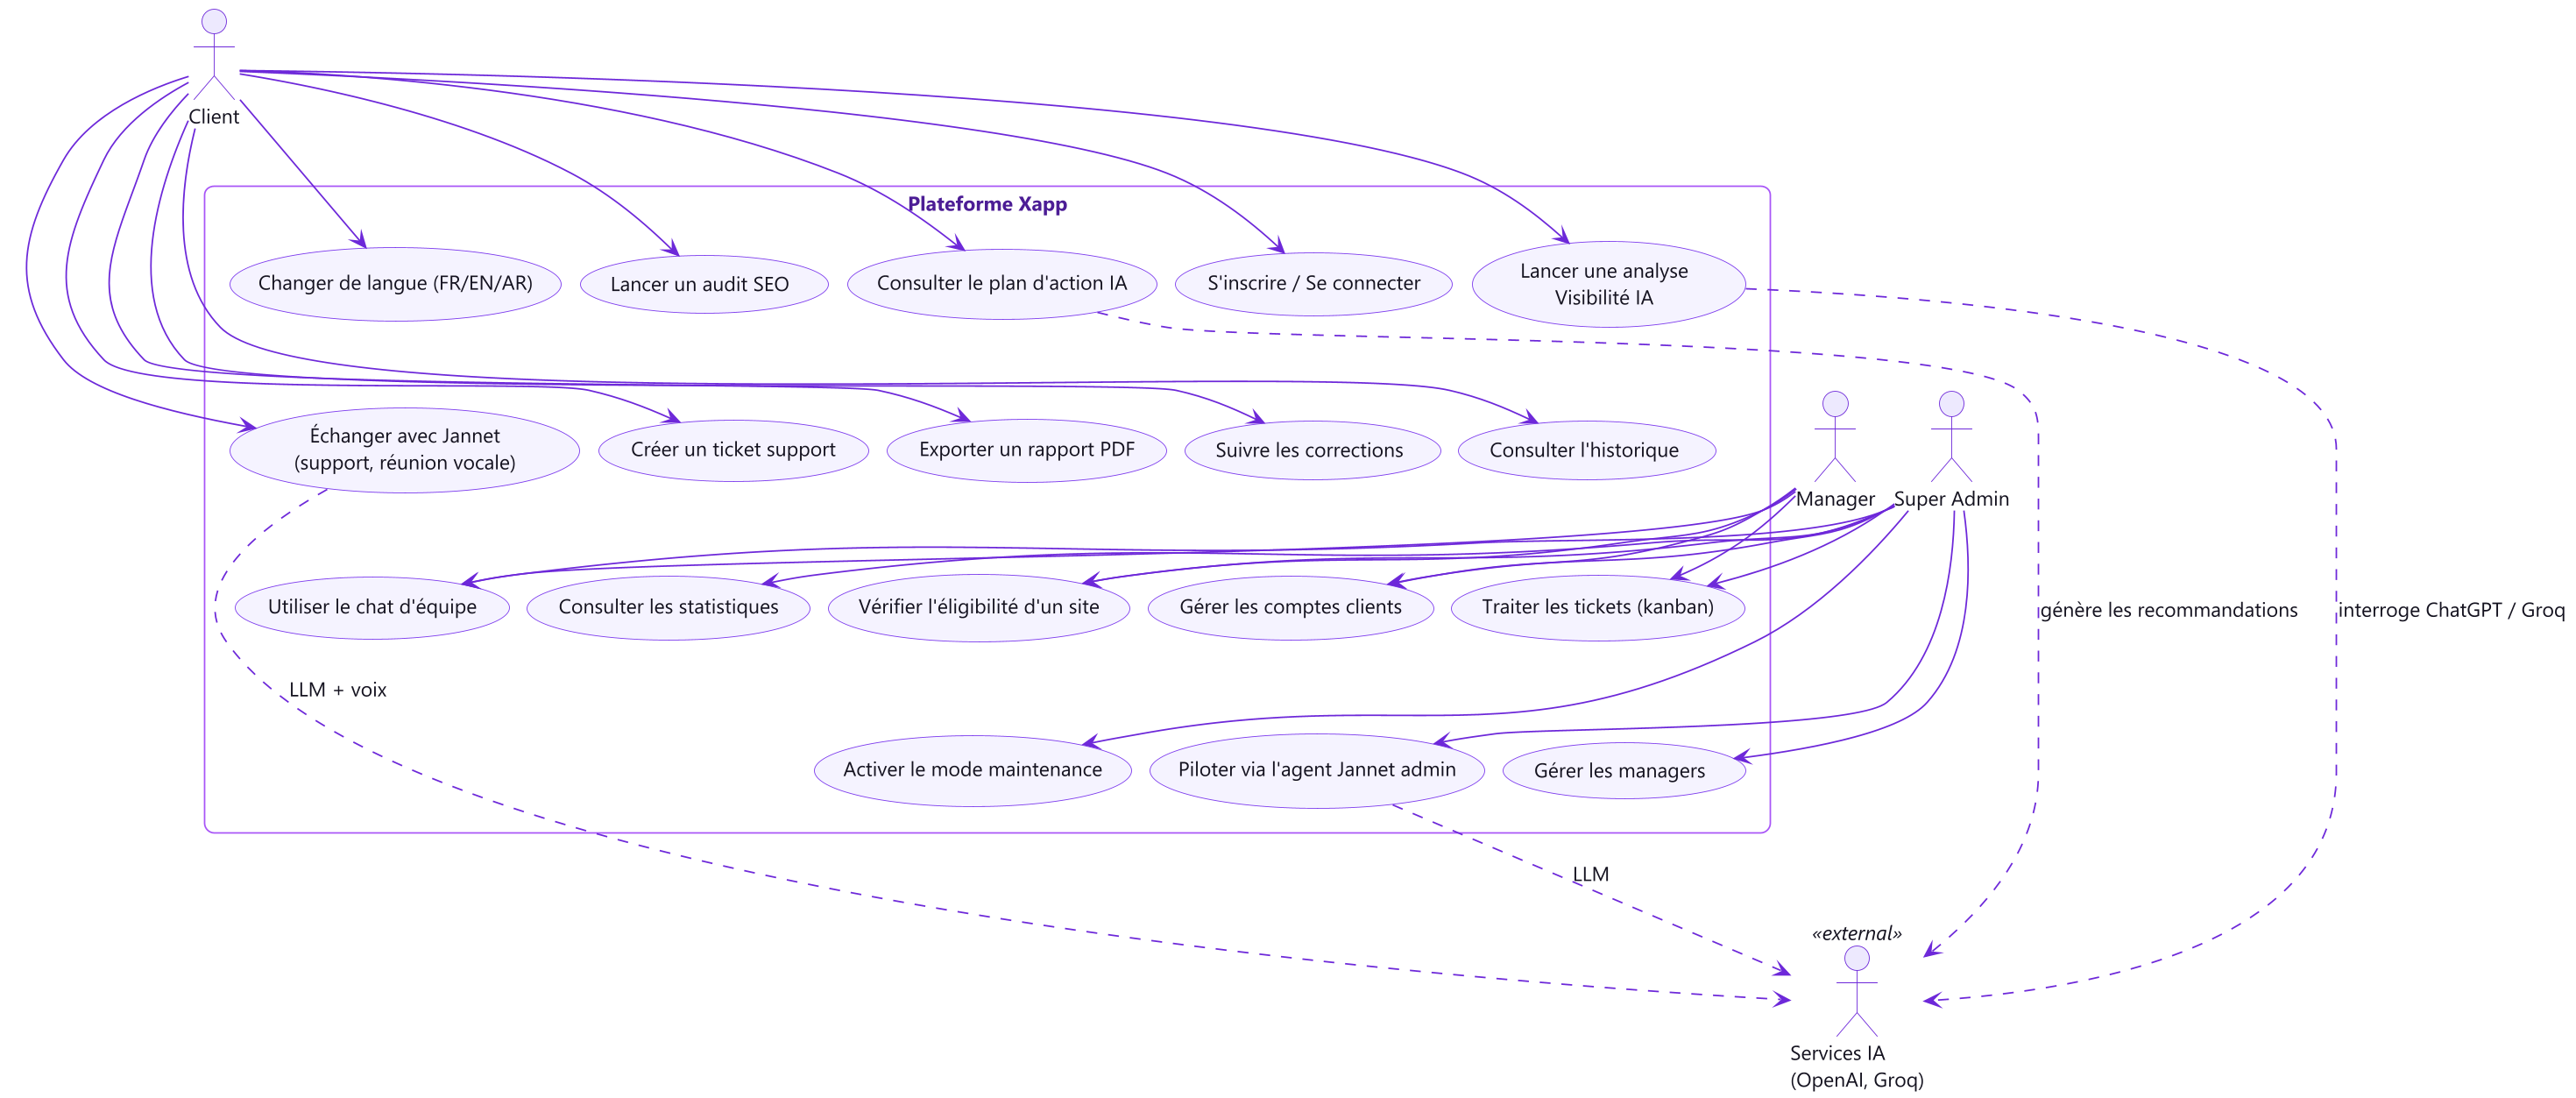
\includegraphics[width=\textwidth,height=0.8\textheight,keepaspectratio]{figures/uml/use_case.png}
  \caption{Diagramme de cas d'utilisation général de la plateforme}\label{fig-cu-global}
\end{figure}

\todo{vérifier que le diagramme de cas d'utilisation reste lisible à l'impression ; sinon le passer sur une page à l'italienne ou le découper par acteur}

\section{Planification par sprint et backlog}
Le backlog du produit a été construit à partir des modules du cahier des charges. Chaque entrée est une histoire utilisateur courte, rattachée à un sprint. Le \cref{tab-backlog} en donne les éléments principaux ; les détails de chaque sprint sont repris dans les chapitres suivants.

\begin{table}[htbp]
\centering
\small
\caption{Backlog du produit (extrait par sprint)}\label{tab-backlog}
\begin{tabularx}{\textwidth}{@{}lXl@{}}
\toprule
\textbf{Sprint} & \textbf{Histoire utilisateur} & \textbf{Priorité}\\
\midrule
\multirow{4}{*}{1} & En tant que visiteur, je veux créer un compte et confirmer mon e-mail & Haute\\
 & En tant qu'utilisateur, je veux me connecter et retrouver mon espace selon mon rôle & Haute\\
 & En tant qu'utilisateur, je veux réinitialiser mon mot de passe par un code reçu par e-mail & Moyenne\\
 & En tant qu'administrateur, je veux créer, modifier et supprimer des comptes & Haute\\
\midrule
\multirow{5}{*}{2} & En tant que client, je veux auditer la page d'accueil de mon site gratuitement & Haute\\
 & En tant que client Pro, je veux auditer tout mon site sans attendre devant l'écran & Haute\\
 & En tant que client, je veux un score sur 100 détaillé par catégorie et par page & Haute\\
 & En tant que client, je veux comparer mon site à mes concurrents & Moyenne\\
 & En tant que client, je veux exporter un rapport PDF & Moyenne\\
\midrule
\multirow{4}{*}{3} & En tant que client, je veux savoir si ChatGPT cite mon site & Haute\\
 & En tant que client, je veux un score AEO/GEO et des recommandations & Haute\\
 & En tant que client, je veux un plan d'action sur deux semaines & Haute\\
 & En tant que client, je veux vérifier qu'une correction est prise en compte & Haute\\
\midrule
\multirow{5}{*}{4} & En tant que client, je veux poser mes questions à un assistant et ouvrir un ticket & Moyenne\\
 & En tant que client, je veux discuter à voix haute de mon audit & Basse\\
 & En tant que manager, je veux traiter les tickets sur un tableau Kanban & Moyenne\\
 & En tant qu'administrateur, je veux confier des actions à un agent IA et pouvoir les annuler & Moyenne\\
 & En tant que client, je veux acheter des crédits en dinars & Haute\\
\bottomrule
\end{tabularx}
\end{table}

\section{Maquettes}
Les maquettes ont porté sur trois écrans clés : la page d'accueil, le tableau de bord et la page d'audit. Une charte graphique commune a été fixée dès le départ : fond sombre pour la navigation, violet comme couleur d'accent (reprise du logo \xapp), cartes arrondies pour le contenu et jauges circulaires pour les scores. \todo{si des maquettes Figma ou papier existent, ajouter ici 2 ou 3 figures (landing, tableau de bord, audit) ; sinon conserver ce paragraphe et le mentionner honnêtement au jury}

\section{Conclusion}
À l'issue du sprint~0, nous disposons d'un périmètre clair : six des sept modules du cahier des charges sont réalisés et le module de monétisation l'est partiellement, auxquels s'ajoute un ensemble d'outils de collaboration. Le chapitre suivant décrit l'architecture technique qui doit les porter.
